% \documentclass[9pt,t]{beamer}
\usefonttheme{professionalfonts}
\usefonttheme{serif}
\PassOptionsToPackage{pdfpagemode=FullScreen}{hyperref}
\PassOptionsToPackage{usenames,dvipsnames}{color}
% \DeclareGraphicsRule{*}{mps}{*}{}
\usepackage{linalgjh}
\usepackage{present}
\usepackage{directories} % defines \vsdir, \vsmpdir
\usepackage{xr}\externaldocument{\vsdir vs1} % read refs from .aux file
\usepackage{catchfilebetweentags}
\usepackage{etoolbox} % from http://tex.stackexchange.com/questions/40699/input-only-part-of-a-file-using-catchfilebetweentags-package
\makeatletter
\patchcmd{\CatchFBT@Fin@l}{\endlinechar\m@ne}{}
  {}{\typeout{Unsuccessful patch!}}
\makeatother

\mode<presentation>
{
  \usetheme{boxes}
  \setbeamercovered{invisible}
  \setbeamertemplate{navigation symbols}{} 
}
\addheadbox{filler}{\ }  % create extra space at top of slide 
\hypersetup{colorlinks=true,linkcolor=blue} 

\title[Spaces and their subspaces] % (optional, use only with long paper titles)
{Spaces and their subspaces}

\author{\textit{Linear Algebra}, edition four \\ {\small Jim Hef{}feron}}
\institute{
  \texttt{http://joshua.smcvt.edu/linearalgebra}
}
\date{}


\subject{Spaces and their subspaces}
% This is only inserted into the PDF information catalog. Can be left
% out. 

\begin{document}
\begin{frame}
  \titlepage
\end{frame}

% =============================================

% ..... Two.I.2.19 .....
\section{Real three-space}
\begin{frame}{Subspaces of $\Re^3$}
The next slide shows a sample of subspaces of the vector space~$\Re^3$:
the entire space, planes, lines, and the trivial subspace.
Subsets are drawn connected to supersets, on the levels 
directly above and below.

On the level one up from the bottom, the subspaces are lines 
(in the second and third case, because
the conjunction of the two conditions means that each is the 
intersection of two planes).
That is, they are one-dimensional.

On the next level up, the subspaces are planes, two-dimensional.
On the top level, the space is $3$-space.
\end{frame}

\begin{frame}
{\centering\includegraphics{asy/r3_subspaces.pdf}}  
\end{frame}


\begin{frame}{Express subspaces as spans}
\ex This is a subset of $\R^3$.
\begin{equation*}
  P=\set{\colvec{x \\ y \\ z}\suchthat x+y+z=0}
\end{equation*}
Here are three members of this set, and an equation showing that the third is a linear combination of the first two,
illustrating that it is a vector space.
\begin{equation*}
  \vec{v}_1=\colvec{1 \\ 2 \\ -3},
  \vec{v}_2=\colvec{-2 \\ -5 \\ 7},
  \vec{v}_3=\colvec{1 \\ 1 \\ -2},
  \qquad
  3\vec{v}_1+\vec{v}_2=\vec{v}_3
\end{equation*}

To get a more useful description, 
take the condition $x+y+z=0$ to be a one-equation linear system
and parametrize.
\begin{equation*}
  P=\set{\colvec{-y-z \\ y \\ z}\suchthat y,z\in\Re}
   =\set{\colvec{-1 \\ 1 \\ 0}y+\colvec{-1 \\ 0 \\ 1}z\suchthat y,z\in\Re}
\end{equation*}
Thus the plane is the span of those two vectors.
\end{frame}
\begin{frame}
The subspace~$P\subseteq\R^3$ is
a plane passing through the origin. 
\begin{center}
  $P=\spanof{\,\set{\colvec{-1 \\ 1 \\ 0}, 
            \colvec{-1 \\ 0 \\ 1}}\,}$
  \qquad
  \vcenteredhbox{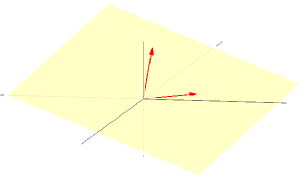
\includegraphics{asy/two_i_a_plane.pdf}}
\end{center}
The two vectors from the spanning set 
\begin{equation*}
  \colvec{-1 \\ 1 \\ 0} 
  \quad\text{and}\quad 
  \colvec{-1 \\ 0 \\ 1}
\end{equation*}
are in red.
For each, its entire body lies in the plane.
\end{frame}



\begin{frame}
\ex 
For the plane
\begin{equation*}
  \hat{P}=\set{\colvec{x \\ y \\ z}\suchthat x+2z=0}
\end{equation*}
repeat the process
\begin{equation*}
  \hat{P}=\set{\colvec{-2z \\ y \\ z}\suchthat y,z\in\Re}
         =\set{\colvec{0 \\ 1 \\ 0}y+\colvec{-2 \\ 0 \\ 1}z\suchthat y,z\in\Re}
\end{equation*}
to express it as a span.
\begin{equation*}
  \hat{P}=\spanof{\,\set{\colvec{0 \\ 1 \\ 0},
                         \colvec{-2 \\ 0 \\ 1}}\,}
\end{equation*}

\pause
\ex
The $xy$-plane is a span in a natural way.
\begin{equation*}
  \text{$xy$~plane}=\spanof{\,\set{\colvec{1 \\ 0 \\ 0},
                                   \colvec{0 \\ 1 \\ 0}}\,}
\end{equation*}
\end{frame}



\begin{frame}
\ex
Next we parametrize the lines.
The conditions in the set description
\begin{equation*}
  L=\set{\colvec{x \\ y \\ z}\suchthat \text{$x-y+z=0$ and $x+2z=0$}}
\end{equation*}
make a linear system.
\begin{equation*}
  \begin{linsys}{3}
    x &- &y &+ &z  &= &0 \\
    x &  &  &+ &2z &= &0
  \end{linsys}
  \grstep{-\rho_1+\rho_2}
  \begin{linsys}{3}
    x &- &y &+ &z  &= &0 \\
      &  &y &+ &z  &= &0
  \end{linsys}
\end{equation*}
Parametrizing
\begin{equation*}
  L=\set{\colvec{x \\ y \\ z}\suchthat \text{$y=-z$ and $x=-2z$}}
\end{equation*}
gives this.
\begin{equation*}
  L=\set{\colvec{-2 \\ -1 \\ 1}z\suchthat z\in\Re}
   =\spanof{\,\set{\colvec{-2 \\ -1 \\ 1}}\,}
\end{equation*}
\end{frame}
\begin{frame}
Here the line, the subspace, is  in yellow. 
In red is the vector used in the description. 
\begin{center}
  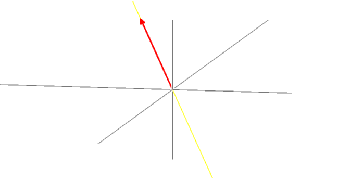
\includegraphics{asy/two_i_a_line.pdf}
\end{center}
In red is the vector used in the description.
\begin{equation*}
  \colvec{-2 \\ -1 \\ 1}
\end{equation*}
Its endpoint lies behind the plane of the screen, in the
octant where $x$ and~$y$
are negative and $z$ is positive.
\end{frame}


\begin{frame}
\ex
The line
\begin{equation*}
  \hat{L}=\set{\colvec{x \\ y \\ z}\suchthat \text{$y=2x$ and $z=0$}}
\end{equation*}
is easy to describe in a parametrized way.
\begin{align*}
  \hat{L} 
  &=\set{\colvec{1/2 \\ 1 \\ 0}y\suchthat y\in\Re}  \\
  &=\spanof{\,\set{\colvec{1/2 \\ 1 \\ 0}}\,}
\end{align*}

\pause
\ex
The $y$-axis is also easy to describe as a span.
\begin{equation*}
  \text{$y$-axis}
  =\spanof{\,\set{\colvec{0 \\ 1 \\ 0}}\,}
\end{equation*}
\end{frame}


\begin{frame}
\ex 
We can describe the entire space as a span.
\begin{equation*}
  \Re^3=\spanof{\,\set{\colvec{1 \\ 0 \\ 0},
                       \colvec{0 \\ 1 \\ 0},
                       \colvec{0 \\ 0 \\ 1}}\,}
\end{equation*}

\pause
\ex
We can do the same for the trivial subspace.
\begin{equation*}
  \set{\colvec{0 \\ 0 \\ 0}}
  =\spanof{\,\set{}\,}
\end{equation*}
(Remember that a sum of zero-many vectors 
is the zero vector.)
\end{frame}

\begin{frame}{$\Re^3$'s diagram reprised}
The following slide repeats the diagram of $\Re^3$'s subspaces, 
showing the same subspaces.
On this diagram the same subspaces they are described as spans, 
where the spanning set uses a minimal number of vectors.

By `minimal' we mean:~while 
we could describe the $xy$-plane in either of these ways,
\begin{equation*}
  \text{$xy$-plane}
  =\spanof{\,\set{\colvec{1 \\ 0 \\ 0},
                  \colvec{0 \\ 1 \\ 0}}\,}
  =\spanof{\,\set{\colvec{1 \\ 0 \\ 0},
                  \colvec{0 \\ 1 \\ 0},
                  \colvec{2 \\ -1 \\ 0}}\,}
\end{equation*}
the second has an extra vector, so the next slide doesn't use that description.
(We will soon make this precise.)

% \pause\medskip
% Note that 
% the subspaces fall naturally into levels, 
% depending on how many vectors are in a minimal spanning set.
\end{frame}
\begin{frame}
{\centering\includegraphics{asy/r3_subspaces_spans.pdf}}
\end{frame}




%...........................
\section{The space of quadratic polynomials}
\begin{frame}{$\polyspace_2$'s subspaces}
The next slide has a picture of some of the subspaces of the
space of quadratic polynomials.
As with the $\Re^3$ diagram, 
subsets are shown connected to supersets on the adjacent level.

With $\Re^3$ the geometry gave us a good start for a natural classification
of subspaces into planes, lines, etc.
In this space there is less of that sense.
But there are a couple of natural subspaces.
\begin{align*}
  \text{linear polynomials}
    &=\set{0x^2+bx+c\suchthat b,c\in\Re}  \\
  \text{constant polynomials}
    &=\set{0x^2+0x+c\suchthat c\in\Re}  
\end{align*}
These are on the next slide, 
along with a couple of more-generic spaces.
\end{frame}
\begin{frame}
{\centering\includegraphics{asy/p2_subspaces.pdf}}  
\end{frame}


\begin{frame}{Parametrizing}
\ex
For the top level, this will do.
\begin{equation*}
  \polyspace_2
  =\spanof{\,\set{x^2,x,1}\,}
  =\spanof{\,\set{x^2+0x+0,
               0x^2+x+0,
               0x^2+0x+1}\,}       
\end{equation*}

\ex
On the bottom level, 
the trivial subspace is the span of the empty set.
\begin{equation*}
  \set{0}
  =\set{0x^2+0x+0}
  =\spanof{\,\set{}\,}
\end{equation*}

\pause
\ex
The set of linear polynomials has a natural expression as a span.
\begin{equation*}
 \set{bx+c\suchthat b,c\in\Re}
  =\spanof{\,\set{x,1}\,}
\end{equation*}

\ex
The set of constant polynomials is similar.
\begin{equation*}
  \set{0x^2+0x+c\suchthat c\in\Re}
  =\spanof{\,\set{1}\,}
\end{equation*}
\end{frame}


\begin{frame}
\ex
Parametrize $P=\set{ax^2+bx+c\suchthat a+b+c=0}$ 
in much the same way as for subspaces of real three-space:
treat the restriction as a one-equation linear system and parametrize.
\begin{align*}
  % \set{ax^2+bx+c\suchthat a+b+c=0}
  P
  &=\set{ax^2+bx+c\suchthat a=-b-c}     \\
  &=\set{(-b-c)\cdot x^2+bx+c\suchthat b,c\in\Re}  \\     
  &=\set{(-x^2+x)\cdot b+(-x^2+1)\cdot c\suchthat b,c\in\Re}       
\end{align*}
The spanning set is $\set{-x^2+x, -x^2+1}$.

\pause
\ex
Simliarly for 
$\hat{P}=\set{ax^2+bx+c\suchthat \text{$a-c=0$ and $b-c=0$}}$.
\begin{align*}
  \hat{P}
  &=\set{ax^2+bx+c\suchthat \text{$a=c$ and $b=c$}}     \\
  &=\set{cx^2+cx+c\suchthat c\in\Re}     \\
  &=\set{(x^2+x+1)\cdot c \suchthat c\in\Re}       
\end{align*}
The spanning set is $\set{x^2+x+1}$.

\pause\medskip
The next slide reprises $\polyspace_2$'s diagram,
with the subspaces described as spans.
\end{frame}
\begin{frame}
{\centering\includegraphics{asy/p2_subspaces_spans.pdf}}  
\end{frame}


\section{Putting the examples together}
\begin{frame}
  \frametitle{Summary}

Subspaces are naturally described as spans.
In both examples these spans fall naturally into levels, 
according to the 
number of elements in a minimal spanning set. 

The book's next section gives a precise definition of 
when a spanning set is `minimal'.
The section after that shows that for any space, 
two minimal spanning sets have the same number of vectors.
\end{frame}

%...........................
% \begin{frame}
% \ExecuteMetaData[../gr3.tex]{GaussJordanReduction}
% \df[def:RedEchForm]
% 
% \end{frame}
\end{document}
